\section{Einleitung}
\label{sec:Einleitung}
Mithilfe dieses Versuchs wird das Relaxationsverhalten beim Entladevorgang
eines Kondensators in einem RC-Tiefpass auf sein Frequenzverhalten, auch bei
hohen Frequenzen, und die Phasenverschiebung zwischen der Kondensator- und der
Generatorspannung hin untersucht. Weiterhin wird die Eigenschaft, nach welcher
der Tiefpass als Integrator verwendet werden kann, betrachtet.
\section{Theorie}
\label{sec:Theorie}
Der Vorgang der Relaxation eines Systems ist dadurch beschrieben, dass es nach Verlassen seines
Ausgangszustands wieder nicht-oszillatorisch in denselben zurückkehrt.\newline
Als hier im Versuch näher betrachtetes Beispiel für eine Relaxation wird der Auf- und Entladevorgang eines Kondensators in einem
RC-Glied, wie exemplarisch in Abbildung \ref{fig:bild1} zu sehen, gewählt.
\begin{figure}[H]
  \centering
  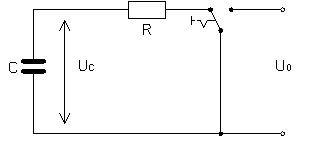
\includegraphics[scale=1.0]{bilder/bild11.png}
  \caption{Schaltung eines RC-Glieds.}
  \label{fig:bild1}
\end{figure}
Für den Aufladevorgang folgt aus den Kirchhoffschen Gesetzen und aus der Betrachtung der beiden Randbedingungen
\begin{align}
Q(0)&=0 & Q(\infty)&=CU_0,
\label{eq:RB}
\end{align}
dass sich für diesen Fall eine Beziehung der Form
\begin{equation}
Q(t)=CU_0 \Bigl(1-e^{\frac{-t}{RC}}\Bigr)
\label{fig:aufladen}
\end{equation}
ergibt.\newline
Hier und im Folgenden ist C die Kapazität des Kondensators, R der Wert des Widerstands und Q(0) die Ladung zum Zeitpunkt t=0.\newline
Der zeitliche Verlauf der Entladung des Kondensators kann durch
\begin{equation}
Q(t)=Q(0) \Bigl(1-e^{\frac{-t}{RC}}\Bigr)
\label{eq:entladen}
\end{equation}
beschrieben werden.\newline
Die Zeitkonstante RC gibt hierbei an wie schnell das System in den Endzustand Q(\infty) relaxiert.\newline

Des Weiteren lassen sich Analogien zu mechanischen Systemen finden.\newline
Wird ein solches mit einer Kraft mit seiner Frequenz angeregt,
so steht es in direktem Bezug zu einem angeregten RC-Kreis.\newline
Somit lässt sich der RC-Kreis als globales Beispiel betrachten, dessen Verhalten auf andere Bereiche, wie der Mechanik, übertragen werden können.
So können zum Beispiel Parallelen in den Schwingungsgleichungen selber und im Verhalten bei einem Widerstand gefunden werden.
\begin{figure}[H]
  \centering
  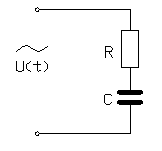
\includegraphics[scale=1.0]{bilder/bild22.png}
  \caption{Schaltung eines angeregten RC-Glieds.}
  \label{fig:bild2}
\end{figure}
Unter Betrachtung eines RC-Kreises, der mit einer Wechselspannung
\begin{equation*}
  U(t)=U_0\cos(\omega t)
\label{eq:angeregt}
\end{equation*}
angeregt wird, kann bemerkt werden, dass eine Phasenverschiebung \phi zwischen der Eingangsspannung und der Spannung
am Kondensator bei zunehmender Frequenz auftritt.\newline
Ist die Frequenz $\omega$ hinreichend gering, also $\omega \ll \frac{1}{RC}$,
so wird die Kondensatorspannung $U_C(t)$ ungefähr gleich der Eingangsspannung $U(t)$ sein.\newline
Durch Erhöhen der Frequenz kann eine Phasenverschiebung zwischen den beiden Spannungen erzwungen werden;
das Auf- und Entladen des Kondensators bleibt über die Zeit gesehen hinter der Generatorspannung zurück.\newline
Als Formel ergibt sich
\begin{equation}
  \phi (\omega) = \arctan(-\omega RC)
\label{eq:phase}
\end{equation}
für die Phasenverschiebung $\phi$ in Abhängigkeit von der Frequenz $\omega$.\newline
Für niedrigere Frequenzen nähert sich die Phasenverschiebung dem Wert 0 an.\newline
Für hohe hingegen tritt eine asymptotische Näherung an $\frac{\pi}{2}$ auf.\newline

Auch kann mithilfe von
\begin{equation}
A(\omega) = \frac{U_0}{\sqrt{1+\omega^2R^2C^2}}
\label{eq:tiefpass}
\end{equation}
festgestellt werden, dass die Amplitude A der Kondensatorspannung bei hohen Frequenzen
abnimmt.\newline
Es gilt, dass aus $\omega \to 0$  folgt, dass $A(\omega)$ gegen $U_0$ geht
und umgekehrt für $\omega \to \infty$ die Amplitude gegen 0 verläuft.\newline
Dieses Verhalten solcher Tiefpässe ist eben dadurch charakterisiert, dass
Frequenzen mit $\omega \gg \frac{1}{RC}$ immer weiter gesperrt und
$\omega \ll \frac{1}{RC}$ durchgelassen werden.\newline
Es lässt sich außerdem zeigen, dass ein solcher RC-Tiefpass unter der Voraussetzung dass $\omega \gg \frac{1}{RC}$,
also die Frequenz sehr groß ist, die zeitlich veränderliche Spannung $U(t)$ integriert.\newline
Es gilt:
\begin{equation}
  U_C(t) = \frac{1}{RC}\int_0^t U(t')\symup{d}t'
  \label{eq:integrator}
\end{equation}
